\documentclass[a4paper,11pt]{article}
\usepackage[utf8]{inputenc}
\usepackage{titling}
\usepackage[a4paper,margin=0.75in]{geometry} % Adjust the margins here
\usepackage{amsmath,amssymb,amsfonts}
\usepackage{algorithmic}
\usepackage{graphicx}
\usepackage{textcomp}
\usepackage{comment}
\usepackage{xcolor}
\usepackage{enumitem}
\usepackage{tcolorbox}
\usepackage{listings}
\tcbuselibrary{listings,skins}  

\usepackage{changepage}

\usepackage{caption}
\usepackage{draftwatermark}
\usepackage{environ}

\usepackage{lmodern} % Optional: Use a scalable font family
\usepackage{scalefnt} % Optional: Allow smooth font scaling

\usepackage{siunitx} % ohm symbol

\usepackage{fancyvrb}     % for the Verbatim environment
% Customize watermark
\SetWatermarkText{\scalefont{1.5}GOWDA} % Use scalefont for scaling
\SetWatermarkScale{.2} % Adjust scale to avoid very large fonts
\SetWatermarkColor[gray]{0.7} % Light gray (80% white)
\SetWatermarkAngle{30}
%\SetWatermarkHorCenter{8cm} % Move right by 3 cm
%\SetWatermarkVerCenter{18cm} % Move up by 12 cm




\newtcblisting{codebox}[2][]{%
  colback=blue!10,           
  colframe=black,                       
  boxrule=1pt,               
  title={#2},                
  listing only,              
  listing engine=listings,   
  listing options={%
    language=Python,
    upquote = true,
    basicstyle=\ttfamily\small,
    breaklines=true,
    showstringspaces=false,
    frame=none,
    xleftmargin=0pt,
    xrightmargin=0pt,
    aboveskip=0pt,
    belowskip=0pt,
    #1
  },
}

\newtcblisting{outputs}[1][]{%
  colback=green!10,
  colframe=black,
  boxrule=1pt,
  title={Output:},
  listing only,
  listing engine=listings,
  listing options={%
    language=Python,
    upquote = true,
    basicstyle=\ttfamily\small,
    commentstyle=\ttfamily\small,
    breaklines=true,
    showstringspaces=false,
    frame=none,
    xleftmargin=0pt, xrightmargin=0pt, aboveskip=0pt, belowskip=0pt,
    columns=fullflexible,
    #1
  },
}

\newtcblisting{syntax}[1][]{%  ← only one optional argument now
  colback=red!10,
  colframe=black,
  boxrule=1pt,
  title={Syntax:},         % ← fixed, constant title
  listing only,
  listing engine=listings,
  listing options={%
    language=Python,
    upquote=true,
    basicstyle=\ttfamily\small,
    breaklines=true,
    showstringspaces=false,
    frame=none,
    xleftmargin=0pt,
    xrightmargin=0pt,
    aboveskip=0pt,
    belowskip=0pt,
    #1                            % any per-box overrides
  },
}


\title{Introduction to Programming \\ Lab: Understanding Loops}
\author{Vikas Thammanna Gowda}
\date{07/29/2025}

\lstset{
    language=Python,
    basicstyle=\ttfamily\small,
    keywordstyle=\bfseries,
    showstringspaces=false,
    breaklines=true,
    frame=none,
    xleftmargin=5pt,
    xrightmargin=5pt,
    aboveskip=10pt,
    belowskip=5pt,
    captionpos=b
}
\begin{document}
\maketitle

\noindent \textbf{Name: \_\_\_\_\_\_\_\_\_\_\_\_\_\_\_\_\_\_\_\_\_\_\_\_\_\_\_\_\_\_\_\_\_\_\_\_\_\_\_\_\_\_\_\_\_\_\_}
\section*{Introduction}
In this lab, you will build and program a Raspberry Pi circuit to create two 
lighting projects: a circular LED sequence and a traffic light simulator with pedestrian crossing.

\begin{itemize}
\item \textbf{Part 1:} You will be provided with the \textit{complete code, circuit diagram, setup, 
and wiring instructions}, along with a \textit{brief in-class demonstration}. 
In this part, four LEDs will blink in a loop, one after the other, 
creating the illusion of a moving light.

\item \textbf{Part 2:} A collaborative activity, where you will work in groups to reconfigure 
the circuit to simulate the behavior of a basic traffic light with pedestrian crossing. 
You will modify the code and test your design as a team, 
applying your understanding of loops and GPIO control. 
\end{itemize} 

\subsection*{Learning Objectives}
\begin{itemize}
    \item Understand the purpose and behavior of \texttt{while} loops.

\item Apply \texttt{while (true)} loops to create continuous, repeating LED patterns.

\item Observe how loop structure controls the timing and order of physical outputs.

\item Modify loop contents to change the LED blinking sequence and timing.

\item Use \texttt{sleep()} delays within loops to control the pace of execution.

\item Recognize how loops interact with real-world hardware through GPIO control.

\item Implement \texttt{try} and \texttt{except} blocks to safely exit infinite loops.
\end{itemize}

\subsection*{Required Components:}
\begin{itemize}
    \item Raspberry Pi (any model with 40 GPIO pins) with Raspbian/Raspberry Pi OS installed. 
\item Breadboard and jumper wires.
\item 4 LEDs for Part 1. For Part 2, you’ll specifically use 3 LEDs (one red, one yellow, one green to mimic a traffic light).
\item 4 Resistors (220 $\Omega$ or 330 $\Omega$ are typical) - one for each LED to limit current. 
\item 1 Button
\end{itemize}


\newpage
\section*{Part 1: Four LEDs in a Circular Sequence}
In this part, you will build a circuit with four LEDs and run
the program to turn them on and off in a repeating loop. 
The LEDs will light up one by one in order, creating a chaser 
or “spinning” effect (imagine a single light that appears to move 
from one LED to the next in a circle). This will involve a continuous loop 
(to keep the lights blinking until you stop the program) 
and timing delays to control the speed of the chase.

\subsection*{Illustration}

Follow these steps to assemble the LED circuit. \textbf{Make sure your Raspberry Pi 
is shut down or powered off while wiring the circuit to avoid any accidental 
short circuits or damage.}

\begin{enumerate}
    \item \textbf{Place the LEDs on the breadboard:} Arrange the four LEDs in a roughly circular or square 
        layout on your breadboard (this is just for visual effect, the exact placement isn't
        critical as long as each LED is in a separate row). Ensure the legs of each LED are in 
        different rows so they aren't accidentally connected. Recall that an LED has polarity: 
        the longer leg is the positive anode, and the shorter leg is the negative cathode. 
        The anode will connect to a GPIO pin (through a resistor), and the cathode will 
        connect to the Raspberry Pi's ground. (Tip: If you forget which leg is which, 
        note that the flat side of the LED casing corresponds to the cathode, and the 
        cathode leg is usually shorter.)

    \item \textbf{Add resistors in series with each LED:} Connect one end of a resistor to the anode of each LED. 
        The resistor can go in the same row as the LED's anode lead. 
        The other end of the resistor will later go to a GPIO pin via a jumper wire. 
        Using 220 or 330 $\Omega$ resistors for standard 5mm LEDs will limit the current 
        and protect the LED and GPIO pin. All four LEDs need their own resistor. 
        (It doesn't matter which end of the LED the resistor is on, as long as it's in series - 
        either between GPIO and anode, or between cathode and ground - the effect is the same.)
    
    \begin{figure}[h] % 'h' places the figure approximately here
        \centering
        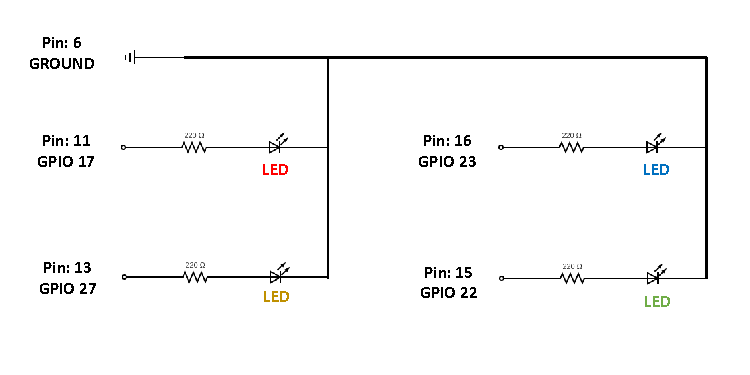
\includegraphics[width=1\textwidth]{fig1.pdf} % Change size as needed
        \caption{Circuit Diagram.}
        \label{fig:runtime}
    \end{figure}

    \item \textbf{Connect LED cathodes to ground:} Connect the negative leg (cathode) of each 
        LED to the Pi's ground. An easy way to do this is to use a ground rail on the breadboard. 
        First, use a jumper wire from one of the Pi's GND pins 
        (there are several GND pins; one convenient GND is physical pin 6 on the GPIO header) 
        to a hole in the breadboard and designate that entire row as “ground”. 
        Then connect a short jumper from each LED's cathode row to that ground rail. 
        Now all LED cathodes are tied to the Pi's ground (they can share the same ground rail since ground is common).

    \item \textbf{Connect LED anodes to GPIO pins:} Now connect the free end of each resistor 
        (the end not connected to an LED yet) to the appropriate Raspberry Pi GPIO output pin using jumper wires. 
        We will use the Broadcom (BCM) numbering for GPIO pins (this is the default numbering system in the 
        gpiozero library). The four GPIO pins we'll use are:
        \begin{itemize}
            \item GPIO17 - physical pin 11 on the Pi's header
            \item GPIO27 - physical pin 13
            \item GPIO22 - physical pin 15
            \item GPIO23 - physical pin 16
        \end{itemize}

        Each resistor end gets one jumper wire to one of these GPIO pins. 
        For example, connect the resistor from LED1's anode to GPIO17, LED2's 
        resistor to GPIO27, LED3's resistor to GPIO22, and LED4's resistor to GPIO23. 
        These four GPIO pins are all on the same side of the header 
        (they are convenient because they are adjacent pins 11, 13, 15, 16). 
        Double-check your connections: each LED's path should be: GPIO pin \textbf{>} resistor -> LED anode, 
        then LED cathode -> ground. If you wire it this way, setting a GPIO 
        pin “HIGH” (on) will forward-bias the LED (current flows from the 3.3V 
        output pin through the LED to ground) and the LED will light. Setting the 
        pin “LOW” (off) will stop current flow, turning the LED off.

    \item \textbf{Final check:} Ensure no two LED leads are accidentally in the same row 
    (which would short them), and verify each LED has one side to ground and one side to 
    a unique GPIO pin (through a resistor). Also ensure your Pi's ground pin is connected 
    to the LED cathodes. The wiring should resemble four “spokes” from the Pi to each LED, 
    with a common ground. Once everything looks correct, you can power on your Raspberry Pi 
    for the next step.

\end{enumerate}

\begin{figure}[h] % 'h' places the figure approximately here
    \centering
    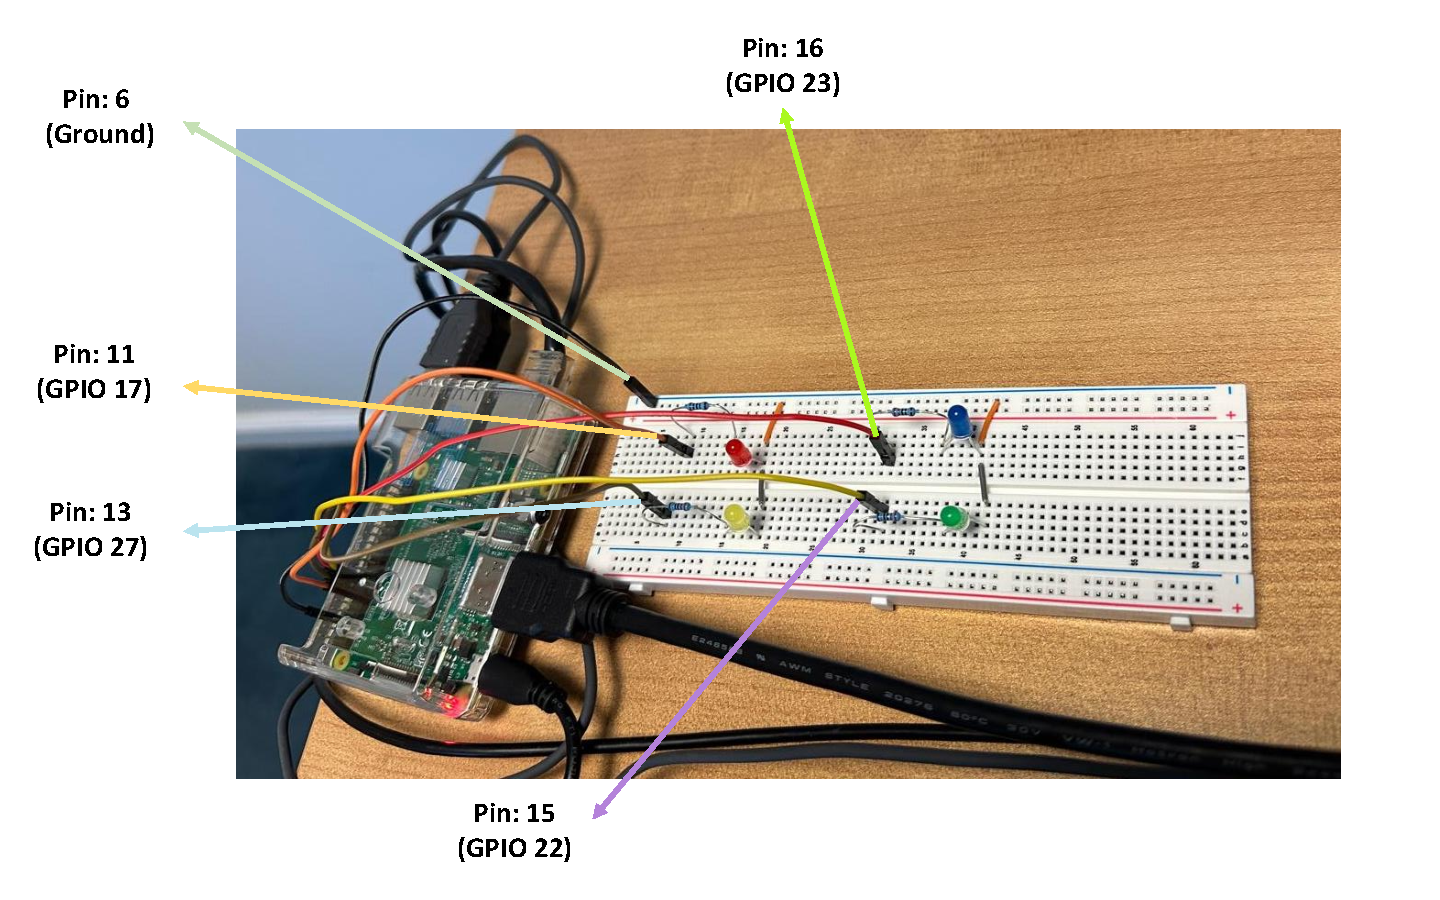
\includegraphics[width=1\textwidth]{fig2.pdf} % Change size as needed
    \caption{Wiring set-up.}
    \label{fig:runtime1}
\end{figure}

\subsection*{Run and Observe}
It’s time to test the circuit and code. Make sure your 
Raspberry Pi is powered on and the circuit is connected as described. 
Run the privided code.

\begin{itemize}
    \item LEDs should light one after another in a circular pattern.
    \item Press \textbf{Ctrl+C} to stop and see “Cleaned up” in the terminal.
\end{itemize}

\newpage
\section*{Part 2: Traffic Light Simulation }
Now that you have mastered basic LED control and looping, let's 
apply those skills to a real-world scenario: a traffic light system.
Real traffic lights cycle through green, yellow (amber), and red lights with specific timing. 
In this part, you will modify your hardware setup to use three 
LEDs—typically one of each color: green, yellow, and red—and update 
your code to simulate a standard traffic signal pattern. 
This exercise demonstrates how the same circuit and code structure can be 
reused and adapted for different purposes simply by changing the sequence and timing logic.

Now, consider how you might enhance this setup by adding a pedestrian crossing button. For instance, when the button is pressed, the traffic light should turn red (if it isn’t already), allowing pedestrians to cross safely.


\subsection*{Circuit Diagram}
Give the circuit diagram:

\newpage
\section*{Reflection and Analysis}
\begin{enumerate}
    \item In your own words, what does while true: do in the program, 
    and why was it used in both parts of this lab? What would happen 
    if we used a for loop with a fixed range instead?

    \item If you wanted the LED chase in Part 1 to run twice as fast, 
    what would you change in the code? Likewise, how would you modify 
    the traffic light timing to make the green light last 10 seconds 
    instead of 5? (Describe which variables or values to change.)

    \item Our programs turn off all the LEDs in the finally block when exiting. 
    Why is this important? What might you observe on the hardware if the program 
    was stopped without turning off the LEDs?

    \item \textbf{Further extension:} Discuss how this project can be extended. 

\end{enumerate}

\end{document}